% This is the Reed College LaTeX thesis template. Most of the work 
% for the document class was done by Sam Noble (SN), as well as this
% template. Later comments etc. by Ben Salzberg (BTS). Additional
% restructuring and APA support by Jess Youngberg (JY).
% Your comments and suggestions are more than welcome; please email
% them to cus@reed.edu
%
% See http://web.reed.edu/cis/help/latex.html for help. There are a 
% great bunch of help pages there, with notes on
% getting started, bibtex, etc. Go there and read it if you're not
% already familiar with LaTeX.
%
% Any line that starts with a percent symbol is a comment. 
% They won't show up in the document, and are useful for notes 
% to yourself and explaining commands. 
% Commenting also removes a line from the document; 
% very handy for troubleshooting problems. -BTS

% As far as I know, this follows the requirements laid out in 
% the 2002-2003 Senior Handbook. Ask a librarian to check the 
% document before binding. -SN

%%
%% Preamble
%%
% \documentclass{<something>} must begin each LaTeX document
\documentclass[12pt,twoside]{reedthesis}
% Packages are extensions to the basic LaTeX functions. Whatever you
% want to typeset, there is probably a package out there for it.
% Chemistry (chemtex), screenplays, you name it.
% Check out CTAN to see: http://www.ctan.org/
%%
\usepackage{graphicx,latexsym} 
\usepackage{amssymb,amsthm,amsmath}
\usepackage{longtable,booktabs,setspace} 
\usepackage{chemarr} %% Useful for one reaction arrow, useless if you're not a chem major
\usepackage[hyphens]{url}
\usepackage{rotating}
\usepackage{natbib}

\usepackage{tikz}
\usetikzlibrary{arrows}
% Comment out the natbib line above and uncomment the following two lines to use the new 
% biblatex-chicago style, for Chicago A. Also make some changes at the end where the 
% bibliography is included. 
%\usepackage{biblatex-chicago}
%\bibliography{thesis}

% \usepackage{times} % other fonts are available like times, bookman, charter, palatino

\title{To Bayes or Not To Bayes: Model Averaging for Bayesian Classifiers}
\author{Brett T. Beutell}
% The month and year that you submit your FINAL draft TO THE LIBRARY (May or December)
\date{May 2014}
\division{Mathematics and Natural Sciences}
\advisor{Irena Swanson}
%If you have two advisors for some reason, you can use the following
%\altadvisor{Your Other Advisor}
%%% Remember to use the correct department!
\department{Mathematics}
% if you're writing a thesis in an interdisciplinary major,
% uncomment the line below and change the text as appropriate.
% check the Senior Handbook if unsure.
%\thedivisionof{The Established Interdisciplinary Committee for}
% if you want the approval page to say "Approved for the Committee",
% uncomment the next line
%\approvedforthe{Committee}

\setlength{\parskip}{0pt}

% From example.net/tikz/examples/red-black-tree
\tikzset{
  treenode/.style = {align=center, inner sep=0pt, text centered,
    font=\sffamily},
  arn_n/.style = {treenode, circle, white, font=\sffamily\bfseries, draw=black,
    fill=black, text width=1.5em},% arbre rouge noir, noeud noir
  arn_r/.style = {treenode, circle, red, draw=red, 
    text width=1.5em, very thick},% arbre rouge noir, noeud rouge
  arn_x/.style = {treenode, rectangle, draw=black,
    minimum width=0.5em, minimum height=0.5em}% arbre rouge noir, nil
}

%%
%% End Preamble
%%
%% The fun begins:
\begin{document}

  \maketitle
  \frontmatter % this stuff will be roman-numbered
  \pagestyle{empty} % this removes page numbers from the frontmatter

% Acknowledgements (Acceptable American spelling) are optional
% So are Acknowledgments (proper English spelling)
    \chapter*{Acknowledgements}
	I want to thank a few people.

% The preface is optional
% To remove it, comment it out or delete it.
 %   \chapter*{Preface}
%	This is an example of a thesis setup to use the reed thesis document class.

    \tableofcontents
% if you want a list of tables, optional
 %   \listoftables
% if you want a list of figures, also optional
  %  \listoffigures

% The abstract is not required if you're writing a creative thesis (but aren't they all?)
% If your abstract is longer than a page, there may be a formatting issue.
    \chapter*{Abstract}
	The preface pretty much says it all.
	
	\chapter*{Dedication}
	You can have a dedication here if you wish.

  \mainmatter % here the regular arabic numbering starts
  \pagestyle{fancyplain} % turns page numbering back on

%The \introduction command is provided as a convenience.
%if you want special chapter formatting, you'll probably want to avoid using it altogether

    \chapter*{Introduction}
         \addcontentsline{toc}{chapter}{Introduction}
	\chaptermark{Introduction}
	\markboth{Introduction}{Introduction}
	% The three lines above are to make sure that the headers are right, that the intro gets included in the table of contents, and that it doesn't get numbered 1 so that chapter one is 1.

% Double spacing: if you want to double space, or one and a half 
% space, uncomment one of the following lines. You can go back to 
% single spacing with the \singlespacing command.
% \onehalfspacing
% \doublespacing
	If it were not for convention, this chapter could perhaps be titled, ``An Irresponsibly Quick Introduction to Bayes' Theorem." It is wholly optional for the reader who has taken an undergraduate course in mathematical statistics. This chapter introduces the ideas, terminology, and some historical minutiae about Bayesian reasoning. Naturally, we provide a statement of Bayes' theorem for events and distributions, and we explore its meaning in an inferential framework. 
	\section{Much Ado About Bayes}
	At its inception, Bayes' theorem was not particularly controversial. Pierre Simon LaPlace offered its first formalization in the early 19th century, and he believed that with a sufficient amount of data, the answers it provided were equivalent to those obtained from his frequency based methods [McGrayne, 2011]. (This belief was ultimately proven wrong in the mid-twentieth century.)
	As time passed, LaPlace preferred his frequentist techniques for the relative ease of their calculations, but he did not outright condemn the use of Bayes in practice. Over a half-century after his death, LaPlace's failure to disown Bayesian reasoning caught the attention of a Scottish mathematician named George Chrystal, who remarked, ``The indiscretions of great men should be quietly allowed to be forgotten" [McGrayne, 2011].
	
	Chrystal's comment represents the attitude of early twentieth century statisticians quite well. At this time, frequentism reigned supreme, and the attitude towards Bayes' theorem and its role in statistics was surprisingly sour. For years, statisticians in the academy who employed Bayesian reasoning feared for their reputation if they explicitly made reference to Bayes' theorem in their work [McGrayne, 2011]. 
	
	Fortunately, with due thanks to the computational advances of the past three decades, Bayes survived its temporary relegation to the catacombs of statistics, and it has emerged as an astoundingly useful tool for the modern statistician. The phrase ``Bayesian Inference" fails to evoke the religious fervor it once did. Furthermore, it is now far more commonplace for statisticians to use both Bayesian and frequentist techniques in their work, tailoring their methods to the problem at hand [Liu et al, 2013].
	
	Summarily, the use of Bayesian reasoning is no longer divisive or taboo, and it is a recent phenomenon that we may begin our inquiry without several pages apologizing for our inferential philosophy. With that said, it does not hurt to quickly consider the differences between a Bayesian and a frequentist. 
		
\section{Bayes'd and Confused}

	Suppose we seek an estimate of a parameter over some set of random variables. We may call said parameter $\theta$ and our random variables (or, {\em data}) $\vec{X}$. We use $\vec{X}$ to talk about our data in the abstract (that is, before they are observed), and we denote a particular set of observed values as $\vec{x}$. 

	We represent the conditional probability of $\theta$ given a set of observed data as $P(\theta | \vec{X} = \vec{x})$. Vice versa, the conditional probability of the data given a fixed $\theta = \theta_0$ can be written $P(\vec{X} | \theta = \theta_0)$. Note that for the former conditional distribution, we are fixing our data and considering $\theta$ a random variable, whereas for the latter, we are doing the converse.

	\subsection*{``To Bayes"}
	Bayesians prefer the former conditional PDF. To a Bayesian, $\theta$ is uncertain, so the best means of knowing more about $\theta$ is directly through the data. Notably, the choice of words here contains an important qualifier; Bayesians want to know ``{\em more}" about $\theta$. Hence, they specify what is already known about the parameter. Similar to the way a mathematician or logician uses axioms, Bayesians find it important to represent in their methods what it is that they already presume to be true.
	
	We can think of a Bayesian model's presumed truths (often called {\em prior beliefs}, the {\em prior distribution} or simply, the {\em prior}) as a starting point, from which data are used to {\em update} the subjective belief about the estimate.  Bayesians use what are called {\em non-informative priors} to approximate a lack of prior knowledge about $\theta$. 
	
	Besides their inherent subjectivity, the essential characteristic of Bayesian methods is that they treat parameters as random variables. Consequently, Bayesian estimates return a probability distribution, which is called the {\em posterior distribution}. The posterior describes the relative likelihoods of different values of $\theta$ given the data and given the {\em a priori} beliefs encoded in the prior distribution.

	\subsection*{``Not To Bayes"}
	For the student of frequentism, the Bayesian approach may lend itself to confusion (or, years ago, anger), since frequentists treat $\theta$ as fixed ($\theta = \theta_0$), and think of their observed data as probabilistic draws that, in the long run, converge to a particular distribution.
	
	Frequentist techniques have two main advantages. Namely, the math involved in their calculations is generally tidy, and their calculations do not require the subjective prior of Bayes' theorem. However, frequentist methods often suffer from having nuanced and unintuitive interpretations. 
	
	For instance, a frequentist p-value in a hypothesis test is a conditional probability that assumes the null hypothesis is true. Hence, it evaluates how probable the observed data would be if $\theta = \theta_0$. On the other hand, a Bayesian p-value would provide the probability of the null hypothesis being true, conditioned on the data. 
	
	To see this symbolically, consider that $P(\vec{X} = \vec{x} | \theta = \theta_0 )$ is, by definition, a statement about the probability of observing $\vec{x}$, given that $\theta = \theta_0$. Frequentists are more apt to talk about the probability of seeing our data, given $\theta$ is a specific value.

\begin{table}[htdp] % begins the table floating environment. This enables LaTeX to fit the table where it works best and lets you add a caption.
\caption[Comparison of Bayesian and Frequentist Reasoning]{A Broad Comparison of Bayesian and Frequentist Methodologies} 
% The words in square brackets of the caption command end up in the Table of Tables. The words in curly braces are the caption directly over the table.
\begin{center}
% makes the table centered
\begin{tabular}{l l l l} 

   &  \textbf{To the Bayesian} & \textbf{To the frequentist} \\ % the first row of the table. Separate columns with ampersands and end the line with two backslashes. An environment begun in one cell will not carry over to adjacent rows.
  \midrule % another horizontal line
\textbf{Parameters are} & Distributions  & Fixed-valued \\ % another row
\textbf{Subjective assessment is} & Essential & Disturbing \\
\bottomrule % yet another horizontal line
\end{tabular}
\end{center}
\label{bvf} % labels are useful when you have more than one table or figure in your document. See our online documentation for more on this.
\end{table}

\section{The First Rule of Bayes' Club}

We introduce a formal, symbolic expression of Bayes' theorem: 

\begin{center}
	$P(A | B) = \displaystyle\frac{P(B | A)P(A)}{P(B)}$,
\end{center}
where $P$ is a function from the set of all possible events, $\Omega$, to $[0,1]$; $A, B \in \Omega$ are events; and $P(\Omega) = 1$. We may also call $\Omega$ the {\em sample space}.

	The proof of Bayes' theorem for events follows quickly from the axioms of probability and the definition of conditional probability. For our purposes, we note that Bayes' theorem also extends to probability distributions. Let $\theta$ be our parameter of interest and $x$ be an observation of a random variable $X$. Let $\pi(\theta)$ be the prior probability distribution on $\theta$, and let $f(X = x | \theta)$ be a density function for $X$. We may then express the posterior as follows:
\begin{center}
	$\pi(\theta | X = x) = \displaystyle\frac{f(x | \theta)\pi(\theta)}{\int_{\theta \in \Theta}f(x |\theta)\pi(\theta)d\theta} \propto f({x} | \theta)\pi(\theta)$,
\end{center}
where $\propto$ denotes proportionality, $\Theta$ is the set of all possible parameter values, and clearly, the denominator is equal to $f(x)$. When the domain of $\theta$ is discrete, we replace the integral in the denominator with a summation.

The above is conventionally presented alongside the pithy, assonant phrase, ``The posterior is proportional to the prior times the likelihood." The numerator of Bayes' theorem is used so frequently that it has its own name, the {\em marginal} of the posterior. Because the denominator, also called the {\em normalization constant}, can be a ghastly integral, it is often more practical to reason about the posterior in terms of its marginal. For example, the denominator of Bayes' theorem disappears from consideration when we compare two possible parameter values given the data. (Not to get ahead of ourselves, but this property of proportionality is also central to running Markov Chain Monte Carlo simulations.)

\section{Classification and Learning}

A classification model is a statistical model where, given some data about an observation, we seek to predict its {\em class}, an unknown categorical variable. We may borrow the language of machine learning and call the predictor variables in our model {\em features}.

Put tersely, classification requires evaluating probability estimates in a decision theoretic framework. That is to say, we estimate the relative probabilities of some datum belonging to each possible class of the unknown categorical variable, and we have a corresponding decision rule that dictates the class to which said datum should be assigned. This all may seem rather abstract, though. So, let us get concrete.

	\subsection*{Example: Spam Email Detection}
	Spam detection is an oft-cited example of classification. It is suitable for our discussion, since it is an area of classification that has benefited greatly from application of Bayes' rule. In a 1998 study, researchers at Microsoft found that filtering emails for spam based off of hard-coded rules was significantly outperformed by even the most reductive of Bayesian classifiers, the aptly-named {\em Na\"{i}ve Bayes} [Sahami et al, 1998]. Here, we use their paper to contextualize what is meant by a classification model. We will continue with this example in the next chapter in order to help characterize Bayesian classifiers. \\ \\
	
	Suppose we have a set of $1,000$ emails, and for each email, we record four pieces of information according to the table below:
	
	\begin{table}[htdp] % begins the table floating environment. This enables LaTeX to fit the table where it works best and lets you add a caption.
\caption[Example Data for Classifications]{Information on a set of 1,000 emails} 
% The words in square brackets of the caption command end up in the Table of Tables. The words in curly braces are the caption directly over the table.
\begin{center}
% makes the table centered
\begin{tabular}{l | l l} 
 \toprule
  \textbf{Variable} & \textbf{Description} \\ % the first row of the table. Separate columns with ampersands and end the line with two backslashes. An environment begun in one cell will not carry over to adjacent rows.
  \midrule % another horizontal line
  Hyperlinks  & A count of the number of hyperlinks in the body of the email \\ % another row
  Domain & The domain of the email's sender (e.g., @reed.edu) \\
  Timestamp & The time at which the email was sent \\
  Spam & Whether or not the email was spam \\
\bottomrule % yet another horizontal line
\end{tabular}
\end{center}
\label{bvf} % labels are useful when you have more than one table or figure in your document. See our online documentation for more on this.
\end{table}

From these data, we can make predictions about whether or not future, incoming emails are spam. If our data were similar to those used by Sahami et al, we may conclude that, say, a message from @reed.edu, sent at noon and containing zero hyperlinks, is unlikely to be spam. On the other hand, an email from @ALL\_UR\_InBoXX-R-beLoNg-2-us.com, which was sent at midnight and contains thirty hyperlinks, would seem a little suspicious. Hopefully, our model would classify it as spam.
	
	\subsection*{A Note on Learning}
	Our method will necessitate data from which we can {\em train} our classification model. That is, in order to use our model, we must first have a set of pre-classified data from which we can estimate our models' parameters. Thus, in the preceding example, we began with a set of $1,000$ emails that had already been classified as either spam or not-spam. From these initial data, we could make a judgement about new, unclassified data. Such an approach is can be described as {\em learning} the parameters of the model.
	
    \chapter{The Bayesian Network}

    	Bayesian Networks are a useful means of visualizing and reasoning about classification models. Put succinctly, a Bayesian Network is a directed acyclic graph (DAG) where each node represents a random variable in the model, and each edge represents a conditional dependency between two random variables.

	\section{Classification at a Glance}

	Suppose we have a set of random variables $V = \{C, X_1, \ldots, X_n\}$, and we seek to predict the value of $C$, a categorical variable, using $X_1, \ldots, X_n$. We call $C$ the {\em class variable}, and we refer to the $X_i$ as the {\em feature variables}. For notational convenience, we may denote the set of feature variables by $\vec{X}$, and we may denote a single set of observed values of $\vec{X}$ as the vector $\vec{x} = (X_1 = x_1, \ldots, X_n = x_n)$.
	\subsection*{The Bayesian Approach}
	Let $C$ have $k$ possible classes. 
	Our goal in a classification setting is to find the probabilities of each class of $C$, given the observed values of the feature variables. Usually (but not always), we seek the value of the class node that maximizes the equation $P(C | \vec{X})$. We appeal to Bayes' theorem:
	\begin{center}
		$P(C = c_i | \vec{X}) = \displaystyle\frac{P(\vec{X} | C = c_i) P(C = c_i)}{\displaystyle\sum_{c_j \in \textrm{dom}\{C\}} P(\vec{X} | C = c_j)P(C=c_j)}$,
	\end{center}
	where $P(\vec{X} | C = c_i)$ is our likelihood function and $P(C = c_i)$ is our prior probability for the class variable when it is equal to $c_i$. Notably, our problem does not require we compute the denominator of the posterior, since
	\begin{center} 
	$\displaystyle\textrm{arg}\max_{c_i \in \textrm{dom}\{C\}}{\{ P(C=c_i | \vec{X} = \vec{x}) \}} = \displaystyle\textrm{arg}\max_{c_i \in \textrm{dom}\{C\}}\{ P(\vec{X} = \vec{x} | C = c_i) P(C=c_i) \}$.
	\end{center}
	To see why, compare the posterior distributions of two possible class values, $c_i$ and $c_j$, given a vector of inputs $\vec{X}$. Assuming these classes have nonzero posterior probabilities, the normalization constant disappears from the following equation:
	\begin{center}
		$\displaystyle\frac{P(C=c_i | \vec{X} = \vec{x})}{P(C=c_j | \vec{X} = \vec{x})} = 
		\displaystyle\frac{\displaystyle\frac{P(\vec{x} | c_i)P( c_i)}{P(\vec{x})}}{\displaystyle\frac{P(\vec{x} | c_j) P( c_j)}{P(\vec{x})}} = \frac{P(\vec{x} | c_i) P( c_i)}{P(\vec{x} | c_j) P( c_j)}$.
	\end{center}
	Clearly, then, if we obtain a value greater than 1 from the above, we find the class $c_i$ to be more likely than $c_j$, given the data. Since the normalization constant $P(\vec{x})$ can be unwieldy to compute, this is a very convenient property of Bayesian classifiers. That is, in this setting, we need only compute the marginal of the posterior for each class.
	\subsection*{Finding the Marginal}
	With a few simple results from probability theory, we can refactor the numerator of the posterior.
	For starters, we invoke the multiplication rule:
	\begin{center}
		$P(\vec{X} | C) P(C) = P(C, X_1, \ldots, X_n)$.
	\end{center}	
	Then, for convenience, we define $X_0 \equiv C$, and we apply the chain rule of probability [[APPENDIX?]] to obtain
	\begin{center}
		$P(X_0,\ldots,X_n) = P( \displaystyle\cap_{i=0}^{n} X_i) = \displaystyle\prod_{j=0}^{n} P(X_j | \displaystyle\cap_{k=0}^{j-1}X_k)$.
	\end{center}
	Thus, our likelihood function requires calculation of all of the conditional dependencies between feature variables in $\vec{X}$, and in order to accurately classify an input $\vec{x}$, we should construct a model that accounts for these conditional dependencies.

	\section{Directed Graphs}
	
	Let $V$ be a set $\{V_0, V_1, \ldots, V_n\}$, and let $E$ be a set of ordered pairs $(V_i, V_j)$ on $V \times V$, (for $n,i,j \in \mathbb{Z}^{+}$). A {\em directed graph} $G$ is defined as the tuple $(V,E)$. We call members of $V$ {\em vertices} or {\em nodes}, and we call members of $E$ {\em edges} or {\em arcs}. Importantly, the order of vertices that compose a particular edge $E_i = (V_j, V_k)$ encodes the {\em direction} of the edge. I.e., $E_i$ is said to be an edge {\em from} $V_j$ {\em to} $V_k$, (for $i,j,k \in \mathbb{Z}^{+})$. Figure 1.1 provides an example of how we might illustrate a directed graph. 	In this context, $V = \{V_0, V_1, V_2\}$ and $E = \{(V_0,V_1),(V_0,V_2),(V_2,V_1)\}$.
	\begin{figure}[htpb]
	\begin{center}
	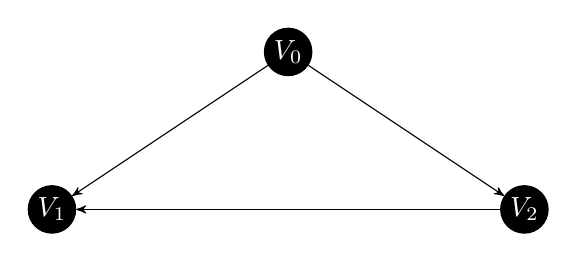
\begin{tikzpicture}[->,>=stealth',level/.style={sibling distance = 5cm/#1, level distance = 1.5cm}] 
  	[scale=.8,auto=left,every node/.style={circle}]
  	\node [arn_n] (n1) at (4,3) {$V_0$};
  	\node [arn_n] (n2) at (1,1)  {$V_1$};
  	\node [arn_n] (n3) at (7,1)  {$V_2$};

	\foreach \from/\to in {n1/n2,n1/n3,n3/n2}
    	  \draw (\from) -- (\to);
	\end{tikzpicture}
	\end{center}
	\caption{A simple directed graph with 3 nodes and 3 edges}
	\label{simple directed graph}
	\end{figure}
	

	\subsection*{Paths and Cycles}
	It is natural to consider the {\em paths} through $G$. A path $P$ of length $n$ is simply an ordered $n$-tuple of edges. 
	We refer to the first and last nodes in this sequence as the {\em starting node} $V_s$ and {\em terminal node} $V_t$, respectively. 
	 With the exception of $V_t$, if the $i^{\text{th}}$ member of $P$ is an edge that points {\em to} the node $V_j$, then the $(i+1)^{\text{th}}$ member is an edge pointing {\em from} node $V_j$ to another node $V_k$. 
	 Thus, a path of length $n$ defines a sequence of $n+1$ nodes, such that each node has an edge from itself to its successor. 
	 By $\mathcal{P}(G)$, let us mean the family of all paths defined on $G$. For any $P \in \mathcal{P}(G)$, we call $P$ a {\em cycle} if $V_s = V_t$. We say that a graph $G$ is {\em cyclic} if there exists at least one cycle in $\mathcal{P}(G)$. Otherwise, we say that $G$ is {\em acyclic}.
	
	\subsection*{Relatives}
	The vocabulary used to describe the relationships amongst nodes in a graph is markedly familial. Given the nodes $V_i, V_j, V_k \in V$, we say that $V_i$ is an {\em ancestor} of $V_j$ if there exists a $P \in \mathcal{P}(G)$ such that $V_i$ precedes $V_j$ in the sequence of nodes defined by $P$. Conversely, we call $V_j$ a {\em descendant} of $V_i$. We also give special names to a node's immediate ancestors and descendants. Formally, for $V_j$, we may define the set of {\em parents} of $V_j$ as $\{V_i : (V_i,V_j) \in E \}$. Similarly, we define the set of {\em children} of $V_j$ as $\{V_k : (V_j, V_k) \in E\}$. A node whose set of parents is empty is called the {\em root node} of our graph.
	
	\subsection*{The Adjacency Matrix}
	We may represent $G=(V,E)$, where $V = \{V_0, \ldots, V_{n-1} \}$ has order $n$, with an $n \times n$ matrix $A = (a_{ij})$, such that for each entry $a_{ij}$, 
	\begin{center}
	 	$a_{ij} = 
		\begin{cases} 1, & \textrm{if\ \ \ } (V_{i-1},V_{j-1}) \in E; \\
		0, & \textrm{otherwise}. \end{cases}$
	 \end {center}
	We refer to $A$ as a {\em binary node-node adjacency matrix} or just an {\em adjacency matrix}. For example, the adjacency matrix corresponding to the first figure of this section would be
	\[
	\begin{pmatrix}
	0 & 1 & 1 \\
	0 & 0 & 0 \\
	0 & 1 & 0
	\end{pmatrix} \]
	since there is an arc from $V_0$ to $V_1$, an arc from $V_0$ to $V_2$, and an arc from $V_2$ to $V_1$. We may also consider the sum of powers of $A$,
	\begin{center}
		$Y = A + A^2 + \cdots + A^n = \displaystyle\sum_{i=1}^{n} A^{i}$.
	\end{center}
	The resulting matrix is $(y_{ij})$, where $y_{ij}$ represents the number of unique paths from $V_s \equiv V_{i-1}$ to $V_t \equiv V_{j-1}$ in $\mathcal P(G)$. 
	Thus, to formalize the notion of an acyclic graph, we say that $G=(V,E)$ is acyclic if $tr(Y) = 0$. 
	Otherwise, $G$ is cyclic.
	To continue our example from above, we would calculate $Y$ to be
	\[
	\begin{pmatrix}
	0 & 2 & 1 \\
	0 & 0 & 0 \\
	0 & 1 & 0
	\end{pmatrix} \]
	which is consistent with our visualization of the graph. 
	(For example, we identify two distinct paths from $V_0$ to $V_1$, and $y_{1,2} = 2$.)
	
	\section{Bayesian Networks}	
	Let $\mathcal{B} \equiv \langle G, \Theta \rangle$, where $G = (V,E)$ is a directed acyclic graph, $V = \{V_0, V_1, \ldots, V_n \}$ is a set of $n + 1$ random variables, and $\Theta$ is a set of parameter estimates corresponding to the structure of $G$. We say that $\mathcal{B}$ is a Bayesian Network.

	\subsection*{Restricted Bayesian Networks}
	A {\em restricted} Bayesian network caps the number of possible conditional dependencies for a given feature variable at some nonnegative integer $k$. Hence, the graph that represents the network should have at most $k$ arcs from each of its feature nodes. The Tree Augmented Network (TAN), displayed below, is an example of a restricted Bayesian Network with $k = 1$.

	\begin{figure}[htpb]
	\begin{center}
	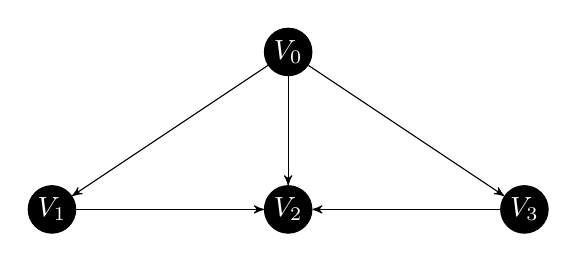
\begin{tikzpicture}[->,>=stealth',level/.style={sibling distance = 5cm/#1, level distance = 1.5cm}] 
  	[scale=.8,auto=left,every node/.style={circle,fill=blue!20}]
  	\node [arn_n] (n1) at (4,3) {$V_0$};	
  	\node [arn_n] (n2) at (1,1)  {$V_1$};
  	\node [arn_n] (n3) at (4,1)  {$V_2$};  	
	\node [arn_n] (n4) at (7,1)  {$V_3$};

	\foreach \from/\to in {n1/n2,n1/n3,n1/n4,n2/n3,n4/n3}
    	  \draw (\from) -- (\to);
	\end{tikzpicture}
	\end{center}
	\caption{TAN with three features}
	\label{simple tan}
	\end{figure}
	 Of course, a Bayesian network without restrictions on its nodes' conditional dependencies is called an {\em unrestricted} Bayesian network.
	
	\section{Bayesian Classifiers}
	A Bayesian classifier is simply a Bayesian network applied to a classification problem.
	We consider the necessary structural and decision theoretic modifications to $\mathcal{B}$ that are necessary for this application.
	
		\subsection*{Networks Constraints}
	In a classification setting, we place a few extra constraints on the graph of $\mathcal{B}$.
	Namely, we may call $V_0$ the class variable, and we may require that the binary node-node adjacency matrix $A$ of $G$ satisfies the following properties:
	\begin{center}
		$\displaystyle\sum_{i=1}^{n}a_{i1} = 0$,\ \ \ and \ \ \ 
		$\displaystyle\sum_{j=1}^{n}a_{1j} \neq 0$.
	\end{center}
	In words, we mean there are no directed edges pointing to the class node, and the class node has an edge to at least one feature node. Obviously, the class node is the root of $G$.
		
		\subsection*{Making a Decision}
	
	To predict the class for an observation, we use a {\em decision rule}.
	Our decision rule provides a means of selecting one proposed classification over another, given a set of pre-classified data and a new input that has yet to be classified.
	Recall that in surveying the general problem of classification, we chose a decision rule that returned the class maximizing our posterior probability. 
	Albeit common, this is not the only possible decision rule. 
	For instance, there may be an unequal cost associated with certain misclassifications of $\vec{x}$. In such cases, we can modify our decision rule's {\em loss function} accordingly; however, this facet of decision theory is not central to our discussion.
	 
	\subsection*{The Naive Bayes Classifier} % \"{} won't compile
	The Na\"{i}ve Bayes classifier (NBC) is highly reductive; yet, it is a surprisingly effective means of classifying data. 
	In essence, we make a simplifying assumption about our data in order to yield a more wieldy computation of the posterior.
	Recall that the posterior distribution of the class variable $C \equiv X_0$ has the following property:
	\begin{center}
		$P(X_0 | X_1, \ldots , X_n) \propto
		P(X_0,\ldots,X_n) = 
		P( \displaystyle\cap_{i=0}^{n} X_i) = 
		\displaystyle\prod_{j=0}^{n} P(X_j | \displaystyle\cap_{k=0}^{j-1}X_k)$.
	\end{center}
	If we assume independence amongst the feature variables $X_1,\ldots,X_n$, then the above simplifies to
	\begin{center}
		$P(X_0) \displaystyle\prod_{j=1}^{n} P(X_j | \displaystyle\cap_{k=0}^{j-1}X_k)
		= P(C) \displaystyle\prod_{j=1}^{n} P(X_j | C)$.
	\end{center}
	Note that our independence assumption makes the NBC's graph a restricted Bayesian network with $k = 0$.
	\subsection*{Example: Spam Detection}
	Let us continue the classification example from section 0.4. Recall that we are given a set of 1,000 emails, pre-classified as either spam or not-spam. Further, for each email, we have information on the sender's domain, the number of hyperlinks in the body of the email, and the time at which the email was sent. 
	
	It is generally easier to learn the parameters of a Bayesian network when the feature variables are categorical. Thus, we might use the domain information to create a variable that indicates whether or not the sender's domain ended in ``.edu." For the count of hyperlinks, we might define categories of Low (0 to 4 hyperlinks), Medium (5 to 10 hyperlinks), and High (more than 10 hyperlinks). Using the timestamp of the emails, we might create an indicator for whether or not an email was sent between midnight and noon. In the end, we could assign our variables to nodes in a graph as follows:

\begin{table}[htdp] % begins the table floating environment. 
\caption[Example Training Data for Na\"{i}ve Bayes Classification]{Variables from the training set of 1,000 emails} 
% The words in square brackets of the caption command end up in the Table of Tables. The words in curly braces are the caption directly over the table.
\begin{center} 
% makes the table centered
\begin{tabular}{c | l l} 
% the tabular environment is used to make the table itself. The {c c c c} specify that the table will have four columns and they will all be center-aligned. You can make the cell contents left aligned by replacing the Cs with Ls or right aligned by using Rs instead. Add more letters for more columns, and pipes (the vertical line above the backslash) for vertical lines. Another useful type of column is the p{width} column, which forces text to wrap within whatever width you specify e.g. p{1in}. Text will wrap badly in narrow columns though, so beware.
\toprule % a horizontal line, slightly thicker than \hline, depends on the booktabs package
  Node &  Variable & Description  \\ % the first row of the table. Separate columns with ampersands and end the line with two backslashes. An environment begun in one cell will not carry over to adjacent rows.
  \midrule % another horizontal line
 $V_0$ & Spam & 1 if Spam; 0 otherwise \\ % another row
 $V_1$ & edu & 1 if from .edu; 0 otherwise \\
 $V_2$ & Hyperlink Count & Low, Medium, or High \\
 $V_3$ & Time & 1 if sent between midnight and noon; 0 otherwise.  \\
\bottomrule % yet another horizontal line
\end{tabular}
\end{center}
\label{inheritance} % labels are useful when you have more than one table or figure in your document. See our online documentation for more on this.
\end{table}
	
Our Na\"{i}ve Bayes classifier would have a graph with the structure depicted in Figure 1.3. Of course, to complete our classifier, we would learn our model parameters from the training set.
	
	\begin{figure}[htpb]
	\begin{center}
	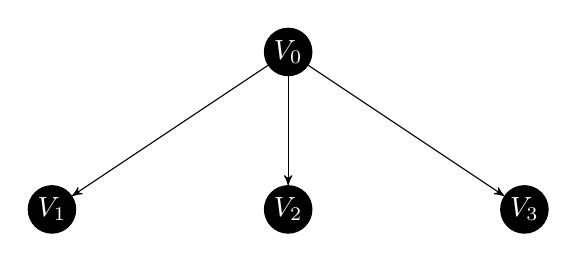
\begin{tikzpicture}[->,>=stealth',level/.style={sibling distance = 5cm/#1, level distance = 1.5cm}] 
  	[scale=.8,auto=left,every node/.style={circle,fill=blue!20}]
  	\node [arn_n] (n1) at (4,3) {$V_0$};	
  	\node [arn_n] (n2) at (1,1)  {$V_1$};
  	\node [arn_n] (n3) at (4,1)  {$V_2$};  	
	\node [arn_n] (n4) at (7,1)  {$V_3$};

	\foreach \from/\to in {n1/n2,n1/n3,n1/n4}
    	  \draw (\from) -- (\to);
	\end{tikzpicture}
	\end{center}
	\caption{A Naive Bayes Classifier} % won't compile with \"{i}
	\label{Example NBC}
	\end{figure}

	\section{Model Structure}
	Unless we have overwhelming prior knowledge that tells us to use a specific graph, we need a means of finding the structure for our Bayesian classifier's network. 
	Sadly, though, the size of the space of all possible network structures is {\em super-exponential} on the number of nodes in a network's graph. 
	Specifically, if $n$ is the number of nodes in a graph, the structure space increases at $2^{O(n^2\log{n})}$ [Koeller, 2001]. 
	Thus, when we have a large number of variables in our model, restricting the number of conditional dependencies in our model is sometimes desirable, as it reduces the size of the structure space. 
	Most importantly, though, we may choose between two modes of reasoning about model structure. 

	\subsection*{Model Selection}	
	The first, called {\em model selection}, involves finding the most probable model structure given our data, which we can then use to estimate our parameters. Generally, this would involve cleverly searching through the space of possible models (or a subset thereof) and ranking structures according to a score function. The structure with the highest score would be our most likely model, and we then would use it to estimate our parameters.  
	
	\subsection*{Model Averaging}
	The second technique, called {\em model averaging} is a little more involved. In lieu of selecting one highly likely model, model averaging would have us make estimates across a space of possible network structures, which are each weighted by their likelihood. Hence, model averaging is a useful tool when we have several model structures that are roughly equiprobable. There are many ways to go about model averaging, and we shall get to one of them in due time. For now, though, it suffices to know that model averaging is computationally very difficult, so we require a means to approximate it by simulation.
	
\chapter{Monte Carlo with Markov Chains}
	The reader may be familiar with Good Old Fashioned Monte Carlo (GOFMC) methods involving independent and identically distributed (IID) data. However, Monte Carlo simulations can also be done with a surprisingly simple stochastic process called Markov Chains. In fact, these Markov Chain Monte Carlo (MCMC) techniques are quite useful for approximating draws from high-dimensional posterior distributions for which we cannot easily find the normalization constant. 
	
	This chapter provides a cursory overview of GOFMC, and then defines Markov chains with the intent of introducing a class of algorithms for Markov Chain Monte Carlo simulation.
	\section{GOFMC}
		\subsection*{An Intuitive Example}
		Imagine we seek to find the area of a peculiar two-dimensional shape called Minnesota. 
		\begin{figure}[h]
	% the options are h = here, t = top, b = bottom, p = page of figures.
	% you can add an exclamation mark to make it try harder, and multiple
	% options if you have an order of preference, e.g.
	% \begin{figure}[h!tbp]
	       	\centering
	    % DO NOT ADD A FILENAME EXTENSION TO THE GRAPHIC FILE
	    	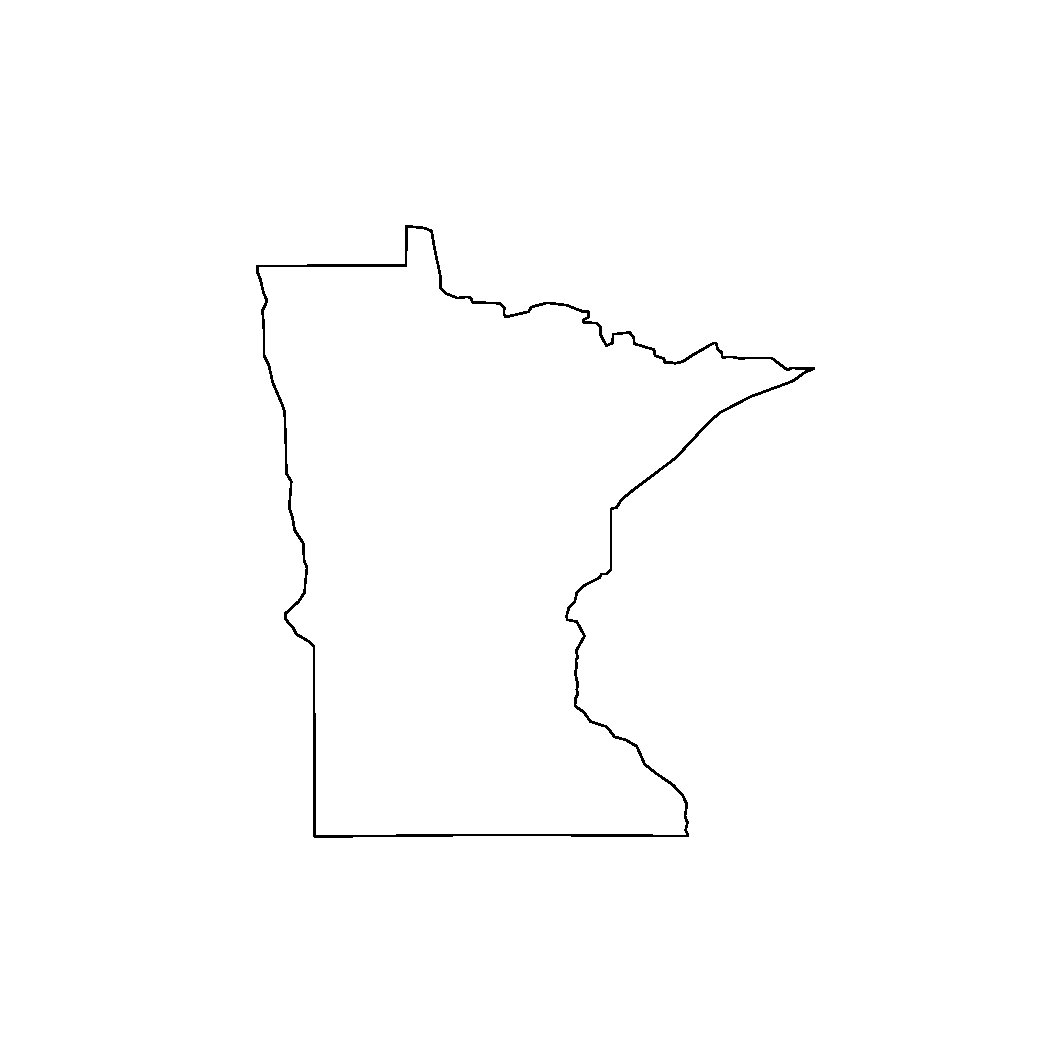
\includegraphics[clip=true, viewport=.3in 1in 6in 6in,scale=0.5]{mn}
	     	\caption{A Two-Dimensional Shape Called Minnesota}
	 	\label{subd}
		\end{figure}	
		We are given no general formula for its area, and all of our attempts to analytically represent the curve that traces its perimeter have proven themselves fruitless. With credit to a talk on Monte Carlo Tree Search given by Peter Drake at the University of Portland, the technique suggested by GOFMC would be the following:
			\begin{enumerate}
				\item Place Minnesota inside a square with edges of known length $s$.
				\item Randomly throw $n$ darts such that they land inside the square. 
				\item Record $x$, the number of darts that landed inside Minnesota.
				\item Multiply the proportion of darts that hit Minnesota ($\frac{x}{n}$) by the area of the square.
			\end{enumerate}
			Symbolically, our GOFMC estimator for the area would be
			\begin{center}
				${s^2} * \displaystyle\sum_{j=1}^{n}\frac{\iota(x_j)}{n}$,
			\end{center}
			where the $x_j$ represent dart-throws, and 
			
			\begin{center}
		 	$\iota(x_j) = 
			\begin{cases} 1, & \text{if the dart hit Minnesota}; \\
			0, & \text{otherwise}. \end{cases}$
			 \end {center}
			The following illustrates our dart-throwing technique from above:
			
			\begin{figure}[h]
		       	\centering
		    	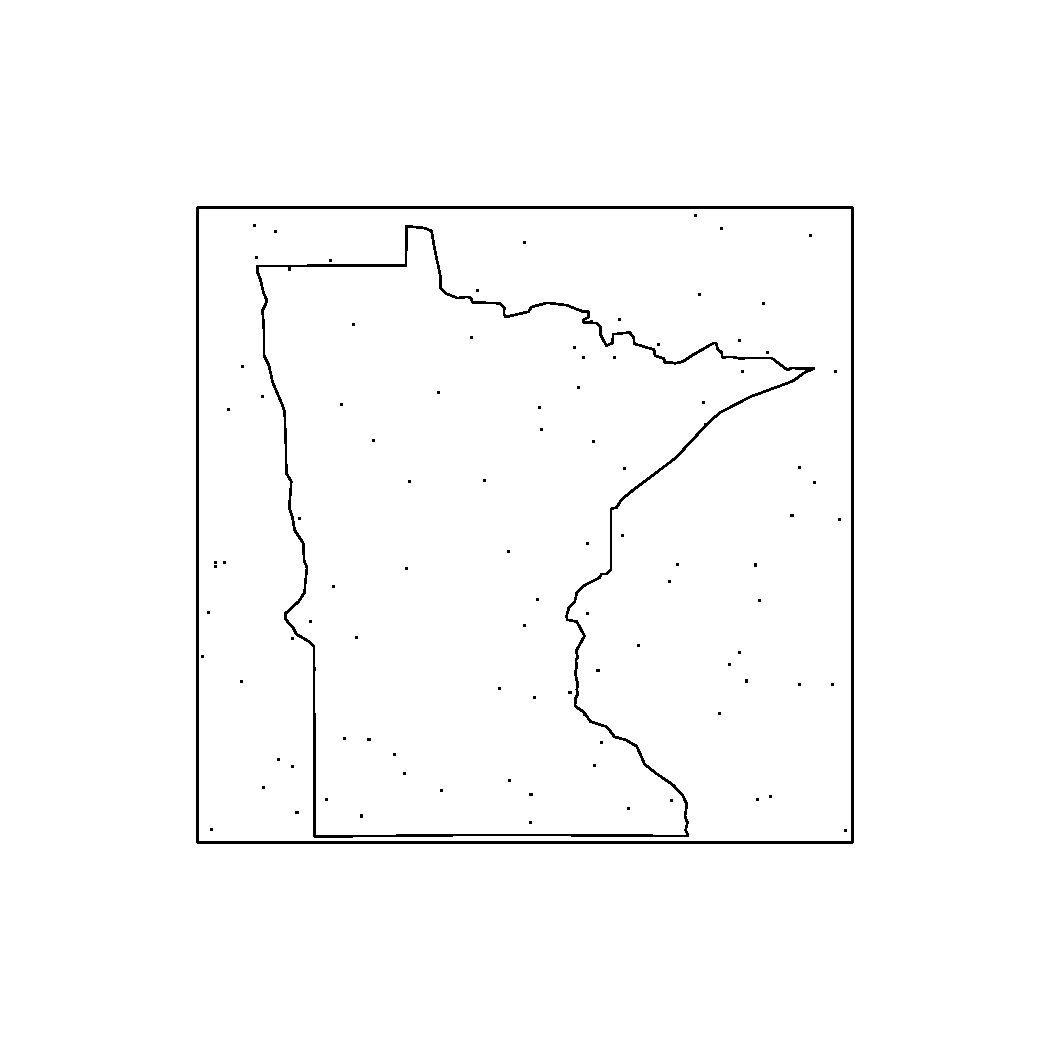
\includegraphics[clip=true, viewport=.3in 1in 6in 6in,scale=0.5]{mn_box_pts}
		     	\caption{Estimating the Area of an Oddly Shaped State}
	 		\label{subd}
			\end{figure}	

			Obviously, our estimate is not exact, but as $n$ approaches infinity, the Law of Large Numbers tells us that we get closer and closer to the true area of Minnesota. Thus is the motivation for GOFMC.
		\subsection*{The General Case}
			Suppose we are given a distribution $\pi$ and we seek to find the expectation of a function $f$ over $\pi$. The central idea of GOFMC is that we may generate IID random variables $X_1, \ldots, X_n$ from $\pi$ in order to estimate $E[f(X_i)]$. A logical estimator, then, by simple application of the method of moments, is 
			\begin{center}
				$\displaystyle\frac{1}{n}\displaystyle\sum_{i=1}^{n}{f(X_i)}$.
			\end{center}		
			Of course, with an estimate comes the corresponding notion of its error. 
			In this case, we define the GOFMC error as
			\begin{center}
				$\epsilon = E[f(X_i)] - \displaystyle\frac{1}{n}\displaystyle\sum_{i=1}^{n}f(X_i)$.
			\end{center}
			By application of the Central Limit Theorem, we know that as $n \rightarrow \infty$, the above converges to a normal distribution with a mean $\mu = 0$ and variance inversely proportional to $n$.
			Hence, with large enough $n$, we can produce fairly accurate estimates from our randomly generated data, and we can have an idea of how erroneous our estimates are. 
	\section{Markov Chains}
	Andrey Markov used his eponymous chain only once in practice, to analyze the occurrence of vowels in a Poeshkin poem \cite{hist}. According to legend, Enrico Fermi ran Markov chains in his head to combat insomnia, but we normal humans tend to reserve such calculations for computers. Thankfully, though, the intuition behind Markov chains is fairly easy to grasp.
	 
	 			\subsection*{Definition}
			Let $s_i$ be a state from a set of possible states (the {\em state space}) $\mathcal S$, and let $I$ be an index set. What we call a {\em Markov chain} $\theta^{(i)}$ is a collection of states from $\mathcal S$ indexed by $i \in I$. Markov chains can be thought of as a sequence of probabilistic transitions from state to state, where the probability of transitioning to the next state in the chain depends solely on the current state. 
			
			Thus, Markov chains have associated {\em transition probabilities}. When $\mathcal S$ is discrete and has finite order $n$, we may specify these probabilities in an $n$ by $n$ {\em transition matrix}, $T = (t_{jk})$, where $t_{jk} = P(\theta^{i+1} = s_k | \theta^{i} = s_j)$. Each row of $T$ admits a probability distribution for a corresponding state in $\mathcal S$. 
			
			Using $T$, we may define a {\em transition function} $p: \mathcal{S}\times\mathcal{S} \rightarrow [0,1]$ on our Markov chain, where $p(s_j,s_k) = t_{jk}$. Consistent with our definition above, $p(s_j,s_k)$ depends solely on $s_j$, and not on any past or future states of the chain. For the sake of concision, we may also refer to transitions as {\em steps}, and when the chain assumes a state $s_j$, we also say that it {\em hits} state $s_j$. 
			
	 
	\subsection*{Example: Andrey the Chameleon}
	To illustrate our definition of Markov chains, we introduce a charismatic chameleon named Andrey. 
	Suppose that Andrey can only assume four distinct colors: blue, green, yellow, or red. Hence, Andrey's state space $\mathcal S$ may be represented as $\mathcal{S} = \{B, G, Y, R\}$. 
	
	We assume that Andrey has no control over the color to which he changes. Instead, the color to which Andrey changes is a probabilistic process, and it only depends on the color that he currently assumes. Andrey's transition matrix $T$ is given by
$$
\bordermatrix{ ~ & B & G & Y & R \cr
	                     B & .25 & .25 & .25 & .25 \cr
	                     G & .8 & .1 & .1 & 0 \cr
	                     Y & .5 & .3 & .02 & .18 \cr
	                     R & 1 & 0 & 0 & 0 \cr	                     	                     	                     
}
$$
	
	For example, $t_{2j}$ is the probability distribution $P(\theta^{i+1} | \theta^i = G)$. That is, if Andrey is currently green, he has an 80\% chance of next turning blue, a 10\% chance of remaining green, a 10\% chance of turning yellow, and a 0\% chance of turning red. 
	
	A possible run of Andrey's associated Markov chain for $1 \leq i \leq 3$ might look like the following:
	\begin{center}
		($\theta^{1} = \textrm{B},\ \  \theta^{2} = \textrm{G},\ \ \theta^{3} = \textrm{B}$).
	\end{center}
	Notice, however, that it would be impossible to observe the following collection of states:
	\begin{center}
		($\theta^{1} = \textrm{B},\ \ \theta^{2} = \textrm{R},\ \  \theta^{3} = \textrm{Y}$),
	\end{center}
	since $p(\textrm{R}, \textrm{Y}) = 0$.
	%Thus, a Markov chain is a series of states, where each state probabilistically transitions to the next state. Most importantly, the transitions only depend on the current state. It thus might help to think of the chain as a stochastic goldfish. I.e., since goldfish are notorious amnesiacs, we can imagine a scenario in which one might swim to the corner of its fishbowl, only to suddenly forget its ultimate trajectory. Hence, all that our forgetful goldfish would know is its current location. Based off of that information, it could stay put, or it could continue moving to another part of the bowl. Once we have a probabilistic description of the goldfish's next move given any position in the tank, we may define a Markov chain.
	%Andrei Markov's first application of his eponymous idea (Markov chains) was to a poem by Poeshkin. Over the next century, others found a wealth of uses for Markov chains. One recent example would be Google, whose idea of a "random surfer" informed their page ranking algorithm [cite the paper!].

		\subsection*{Basic Properties}
		We say a state $s_j \in \mathcal{S}$ is {\em irreducible} if it is possible to get to any other $s_k \in \mathcal{S}$ from $s_j$. If all $s_j \in \mathcal{S}$ are irreducible, the Markov chain $\theta^{(i)}$ over $\mathcal{S}$ is also said to be irreducible. \\
		
		By $Z_i$ we denote the number of steps before a chain hits state $s_i$ once. 
		We refer to this quantity as the {\em recurrence} or {\em hitting time} for state $s_i$.
		We denote the number of steps before a chain hits $s_i$ an arbitrary number of times as $Z^{q}_i$, where $q$ is a positive integer. Clearly, $Z^{q}_i$ is always an integer, and $Z_i$ is simply shorthand for $Z^{1}_i$. We may also define $Z^{0}_i = 0$. \\
		
		Since Markov chains are stochastic processes, $Z^{q}_i$ is a random variable. Hence, we may consider its expectation $E[Z^{q}_i]$. If for all $s_i \in \mathcal S$, the expected hitting time is finite ($E[Z^{1}_i] < \infty$), then we say our Markov chain is {\em positive recurrent}. \\
		
		A Markov chain is {\em periodic} if, for at least one state $s_i$, it can only return to $s_i$ after a number of steps equal to a multiple of some positive integer $k > 1$. Markov chains that contain no periodic states are called {\em aperiodic}. We say a Markov chain is $ergodic$ if it is both aperiodic and positive recurrent. \\
		
		Lastly, the {\em stationary distribution} $\pi$ of a Markov chain is a PDF such that the transition matrix $T$ defined by $\theta^{(i)}$ maintains $\pi$. Symbolically, this looks like the following:
		\begin{center}
			$\displaystyle\sum_{s_j \in \mathcal S} \pi(s_j) * p(s_j,s_k) 
			= \displaystyle\sum_{s_j \in \mathcal S} \pi(s_j) * P(s_k | s_j)
			= \pi(s_k)$.
		\end{center}	
		\section{The Ergodic Theorem}
		The Ergodic Theorem for Markov chains is an analog of the Law of Large Numbers for IID data. It ties together the concepts of aperiodicity, positive recurrence, and the stationary distribution. Importantly, it is through a basic corollary to the Ergodic theorem that we are able to justify use of MCMC in order to estimate draws from intractable distributions.
		\subsection*{Statement}
		Let $\theta^{(i)}$ be an ergodic Markov Chain. 
		Let $V_j(n)$ be defined as follows:
		\begin{center}
			$V_j(n) = \displaystyle\sum_{i=0}^{n-1} \iota_j(\theta^{i})$,
		\end{center}
		where
		\begin{center}
			$\iota_j(\theta^i) = \begin{cases} 
				1, & \textrm{if\ \ \ } \theta^i = s_j; \\
				0, & \textrm{otherwise}. 
				\end{cases}
			$
		\end{center}
		We interpret $V_j(n)$ as the number of visits to state $s_j$ before $\theta^n$ in our Markov chain. 
		Let $E[Z_j] = m_j$ be the expected hitting time of state $s_j$. Then,
		\begin{center}
			$P\left(\displaystyle\frac{V_j(n)}{n} \longrightarrow \frac{1}{m_j}
			\textrm{, as } n \rightarrow \infty \right) = 1$.
		\end{center}
		
		That is, the proportion of times we hit $s_j$ converges in probability to the inverse of the expected recurrence time.
		
		\subsection*{Proof}
		We begin our proof by invoking a result not included herein. Namely, the proportion of times we hit $s_j$ in the chain is the same regardless of the initial state $\theta^0$ of the chain as $n$ goes to $\infty$. Hence, we may fix $s_j$, and without loss of generality, we assume it is the initial state of the chain ($\theta^0 = s_j$). \\
		
		We define $U_{j}^r = Z_{j}^{r} - Z_{j}^{r-1}$. Clearly, then,
		\begin{center}
		 $\displaystyle\sum_{k=1}^{r}U_j^k 
		 = (Z_j^1 - Z_j^0) + \cdots + (Z_j^{r-1} - Z_j^{r-2}) + (Z_j^r - Z_j^{r-1}) 
		 = Z_j^r$. 
		 \end{center}
		 The quantities $U_j^1, \ldots, U_j^r$ are IID random variables, meaning we can find their expectation. Since we may intuitively think of $U_j^r$ as the number of steps between the $(r-1)^{\textrm{th}}$ and $r^{\textrm{th}}$ hits of $s_j$ in our Markov chain, we see that for all $r$,
		\begin{center}
		$E[U_{j}^r] = E[Z_j^{r} - Z_j^{r-1}] = r *E[Z_j] - (r-1) *E[Z_j] = E[Z_j] = m_j$, 
		\end{center}
		which follows from the linearity of expectation.
		Hence, by the Strong Law of Large Numbers [[APPENDIX?]], we get: 
		\begin{center}
		$
		P\left(\displaystyle\frac{\sum_{k=1}^{n}U_j^k}{n} \rightarrow m_j \right) = 1
		$
		\end{center}
		Now, we write
		\begin{center}
		$\displaystyle\sum_{k=1}^{V_j(n)}U_j^k \leq n -1$, 
		\end{center}
		where our sum gives us the number of steps until the last hit of $s_i$ before $\theta^n$ in the chain.
		Obviously, then, the sum could not exceed $n -1$, since we are only considering the number of steps to a state that must occur before the $n^{\textrm{th}}$ step. We may also consider 
		\begin{center}
		$\displaystyle\sum_{k=1}^{V_j(n) + 1}U_j^k \geq n$,
		\end{center}
		where our summation may also be written $Z_j^{V_j(n) + 1}$, which is the number of steps until the first hit of $s_j$ after step $\theta^{n-1}$. 
		Thus, we may squeeze $n$ and divide the resulting inequality by $V_j(n)$.
		\begin{center}
		$$\displaystyle\frac{\displaystyle\sum_{k=1}^{V_j(n)}U_j^k}{V_j(n)} \leq 
		\frac{n}{V_j(n)} \leq 
		\frac{\displaystyle\sum_{k=1}^{V_j(n) + 1}U_j^k}{V_j(n)}$$.
		\end{center}
		Using the convergence in probability of the $U_j^k$ to $m_j$, our sums become
		\begin{center}
		$$\displaystyle\frac{V_j(n) * m_j}{V_j(n)} \leq 
		\frac{n}{V_j(n)} \leq 
		\frac{(V_j(n)+1) * m_j}{V_j(n)}$$,
		\end{center}		
		 and as $n \rightarrow \infty$, we see $\frac{V_j(n) +1 }{V_j(n)} \rightarrow 1$, giving us
		 \begin{center}
		 	$ m_j \leq \displaystyle\frac{n}{V_j(n)} \leq m_j$.
		 \end{center}
		 Hence, as $n \rightarrow \infty$,
		 \begin{center}
		 $$
		 P\left( \displaystyle\frac{n}{V_j(n)} \longrightarrow {m_j} \right) = 1
		 $$
		 \end{center}
		 and we have our result.
		\subsection*{Corollary}
		Given a bounded function $f: \mathcal{S} \rightarrow B$,
		\begin{center}
			$P\left( \displaystyle \frac{1}{n} \sum_{j=0}^{n-1} f(\theta^{j}) 
			= \sum_{s_k \in \mathcal S} \pi(s_k) f(s_k) \right) = 1$, as $n \longrightarrow \infty$.
		\end{center}
		This corollary justifies the use of Monte Carlo methods that estimate expectation of a function over simulated draws from the stationary distribution of our Markov chain.
	\section{MCMC}
			Recall that in the case of GOFMC, we have a distribution $\pi$ from which we can easily simulate random draws, and we then estimate the expectation of a function over $\pi$ through random draws. To perform GOFMC, we must know the PDF for $\pi$. Sometimes, however, we are not so lucky as to be able to fully compute the PDF of our distribution of interest. This occurs frequently in high-dimensional Bayesian analyses, where the denominator of our posterior calculation tends to towards intractability. Thus, we seek an alternative way to simulate draws from $\pi$ when we only know $\pi$ up to a constant. For this, we can use a Markov chain.
		\subsection*{Metropolis Hastings}
			To construct a Markov chain with a stationary distribution equal to our posterior, we must first consider how to transition from state to state. 
			First we need to ensure that the stationary distribution of our chain exists. 
			To that end, we introduce the {\em detailed balance} condition. That is, for all $s_i, s_j \in \mathcal S$,
			\begin{center}
			$ \pi(s_j) p(s_j,s_k) = \pi(s_k) p(s_k,s_j) $
			\end{center}
			This condition is not necessary for the convergence of our chain to the posterior, but it suffices \cite{mcmc}.
			
			Next, we must consider the transition function $p$, which must guarantee that $\pi$ is the unique stationary distribution of our Markov chain. 
			To that end, we split $p$ into a {\em proposal function} ($q: \mathcal S \rightarrow \mathcal S$), which randomly proposes a new state in $\mathcal S$, and an {\em acceptance rule}, which returns the probability that we accept the proposed transition.
			\begin{center}
			$
			p(s_j,s_k) = q(s_j,s_k) \alpha(s_j,s_k)
			$
			\end{center}
			We may assume the proposal function is a random walk with symmetric error.
			Again, this is not wholly necessary, but it suffices for our purposes \cite{mcmc}.
			
			Construction of the acceptance rule is slightly more involved. 
			Essentially, we define a rule that returns a probability of transitioning to the proposed state.
			Suppose we are in state $s_j$, and $q$ proposes a move to state $s_k$. 
			We accept the transition to state $s_j$ with probability equal to
			\begin{center}
			$ \alpha(s_j,s_k) = 
			\begin{cases} \textrm{min}\{1, \frac{\pi(s_k)q(s_j | s_k)}{\pi(s_j)q(s_k | s_j)}\}, & \textbf{if\ \ \ } s_j \neq s_k; \\
			1 - \int q(s_j,s_k)\alpha(s_j,s_k)ds_k, & \textbf{otherwise}. \end{cases}
			$
			\end{center}
			The result is a Markov chain that converges to $\pi$, our posterior distribution.
			
		\subsection*{Sources of Error}
			We face two issues with running Markov chains to approximate the posterior. First, if we sample from the chain directly, our sample is not independent. Hence, taking all of the values from our simulation would not be an IID sample from the posterior. Secondly, the Markov chain converges to the posterior, which means in its early iterations, samples may not approximate the posterior. 
			
			To deal with these issues, we can run a {\em burn-in} period for the chain, and then sample every $n^{\text{th}}$ state of the chain. These are clever heuristics to make our estimates more accurate, but there is little way to quantify how well they perform. Although we know the chain converges to the posterior, we have no theorem which will tell us how many steps in the chain we must take to get an accurate simulation.

\chapter{Bayesian Model Averaging for Bayesian Networks}

	\section{Bayes' Theorem for Models}

	\section{MCMC for BMA}

%If you feel it necessary to include an appendix, it goes here.
    \appendix
      \chapter{Appendix A}
      \section{The Chain Rule for Probability}


%This is where endnotes are supposed to go, if you have them.
%I have no idea how endnotes work with LaTeX.

  \backmatter % backmatter makes the index and bibliography appear properly in the t.o.c...

\newpage
\begin{thebibliography}{1}

\bibitem{msft} M. Sahami, S. Dumais, D. Heckerman, and E. Horvitz. A Bayesian approach to filtering junk email., AAAI Workshop on Learning for Text Categorization, July 1998, Madison, Wisconsin. AAAI Technical Report WS-98-05

\bibitem{mcmc} D. Gamerman and H. F. Lopes. \em{Markov Chain Monte Carlo}. Boca Raton, FL: Chapman \& Hall/CRC, 2006.

\bibitem{hist} S.B. McGrayne. \em{The theory that would not die: How Bayes' rule cracked the enigma code, hunted down Russian submarines, and emerged triumphant from two centuries of controversy}. New Haven, CT: Yale University Press, 2011.

\bibitem{liu} S. Liu, M. Zhu, and Y. Yang. A Bayesian Classifier Learning Algorithm Based on Optimization Model. \em{Mathematical Problems in Engineering}, {2013}. doi: 10.1155/2013/975935. % wtf is DOI?

\bibitem{kiel} N. Friedman and D. Koller. Being Bayesian About Network Structure. Netherlands: Kluwer Academic Publishers, 2000. URL http://robotics.stanford.edu/~koller/Papers/Friedman+Koller:MLJ03.pdf

\end{thebibliography}
% if you're using bibtex, the next line forces every entry in the bibtex file to be included
% in your bibliography, regardless of whether or not you've cited it in the thesis.
%%%    \nocite{*}

% Rename my bibliography to be called "Works Cited" and not "References" or ``Bibliography''
% \renewcommand{\bibname}{Works Cited}

%    \bibliographystyle{bsts/mla-good} % there are a variety of styles available; 
%  \bibliographystyle{plainnat}
% replace ``plainnat'' with the style of choice. You can refer to files in the bsts or APA 
% subfolder, e.g. 
 %%%\bibliographystyle{APA/apa-good}  % or
 %%%\bibliography{thesis}
 % Comment the above two lines and uncomment the next line to use biblatex-chicago.
 %\printbibliography[heading=bibintoc]

% Finally, an index would go here... but it is also optional.
\end{document}
